\documentclass[a4paper,10pt,twocolumn]{article}
\usepackage{amsfonts}
\usepackage{amsmath}
\usepackage{float}
\usepackage{graphicx}
\usepackage{hyperref}
\usepackage{subfigure}

\title{IT2120 - Computer Literacy - FINAL EXAM semester 20201}
\author{Le Minh Duc - 20200164}
\date{\today}

\begin{document}

\twocolumn

\maketitle

\section{How to calculate the score of the test}
\begin{itemize}
\item Complied to pdf file (1 points)
\item Title (0.75 points): each line 0.25 points. It is necessary to have your correct full name and your correct student number.
\item Format the document correctly: class, columns (0.5 points), Sectioning (0.5 points)
\item Format the text correctly (0.5 points)
\item Math (1.5 points): each equation 0.5 points
\item Table (1.5 points)
\item Figure (1.5 points): 0.5 points for the first figure, 1 points for the second figure.
\item Create itemize and enumerate (0.5 points)
\item Cross Ref (0.75 points): 0.25 each.
\item Create table of content 0.5 points
\item Create list of tables 0.25 points
\item Create list of figures 0.25 points
\end{itemize}

\section{Instructions}
\subsection{How to do}
Students need to create this document using latex and follow \textbf{these below rules}:
\begin{enumerate}
\item Need to use ``article'' for document class, a4 paper size, two columns
\item Use commands for sectioning the document, putting the title, author name and date in the title
\item Use cross-referencing commands \texttt{\textbackslash ref}.
\item Command \texttt{\textbackslash mathbb\{N\}} in math environment create character like this $\mathbb{N}$
\item Use package \texttt{hyperref} in your document
\item Put the image file and Latex source file (.tex) in the same folder
\item Text in [\ldots] are to be replaced with your corresponding information.
\end{enumerate}

\subsection{Submission}
Duration: 90 minutes\\
When submission, student need to send to the email address: linhtd@soict.hust.edu.vn\\
Template of email title: [CL2020] - Your Full Name - Your student number.\\
Example: [CL2020] - Nguyen Van A - 20202020.\\
The email needs to have:
\begin{enumerate}
\item Latex source (.tex file).
\item All images inside the document.
\item Output pdf file.
\end{enumerate}
Note: if the Latex file is not compiled, you will be penalized.

\section{Mathematical formulas}
Some notations:
\begin{itemize}
\item $G_w$ denotes a graph containing all vertexes and edges of color $w$.
\item Let's define $w_e$ as follows
\begin{equation}
w_e =
\left\lbrace
\begin{array}{ll}
	100 & \text{if} \ e \  \text{has never been used}\\
	1- f_e/\mathbb{W} & \text{otherwise}
\end{array}
\right.
\end{equation}
\item $(s, d, n)$ denotes a demand to deliver $n$ packages of goods form $s$ to $d$
\end{itemize}
Some related equations:
\begin{equation}
\frac{d^2r_i}{dt^2}= G\sum_{i \neq j} \frac{w_iw_j}{|r_j - r_i|^3}(r_j - r_i)
\label{eqn:sum}
\end{equation}
Replace the value of $w_e$ from 1 to the Equation \ref{eqn:sum} and perform some manipulations, we finally obtain:
\begin{equation}
r_i = \int_{-\infty}^{\infty}f_idt + \int_0^1 f_idt
\end{equation}

\section{Tables and tabulars}
When creating the table, start the basis table and then use the alignment methods. \textbf{Please fill the Table \ref{tab:ttt} with your information.}\\
\begin{table}[h]
\centering
\begin{tabular}{l|l|l}
\hline\hline
\textbf{Not.} & \textbf{Description} & \textbf{Value}\\
\hline
$\mathbb{N}$ & Student name & Le Minh Duc\\
$\mathbb{ID}$ & Student number & 20200164\\
\hline
$g_m$ & Grade of Math exam & 9\\
$g_p$ & Grade of Physics exam & 9\\
$g_e$ & Grade of English exam & 9\\
\hline
\multicolumn{2}{c|}{Final grade = $ \frac{2\times g_m+g_p+g_e}{4}$} & 9\\
\hline\hline
\end{tabular}\caption{Student record}
\label{tab:ttt}
\end{table}

\section{Figures}
Download the images form these addresses:\\
\url{https://users.soict.hust.edu.vn/linhtd/examplelatex.png}\\
\url{https://users.soict.hust.edu.vn/linhtd/figure-topo.pdf}\\
In Figure \ref{fig:rotation}, insert the image into the document so that so that the figures are sidy-by-side and the second one is up side down.
\begin{figure}[H]
\centering

\includegraphics[scale=0.35]{examplelatex.png}
\caption{An example of a Latex document}
\end{figure}

\begin{figure}[H]
\centering
\subfigure[Before]
{
	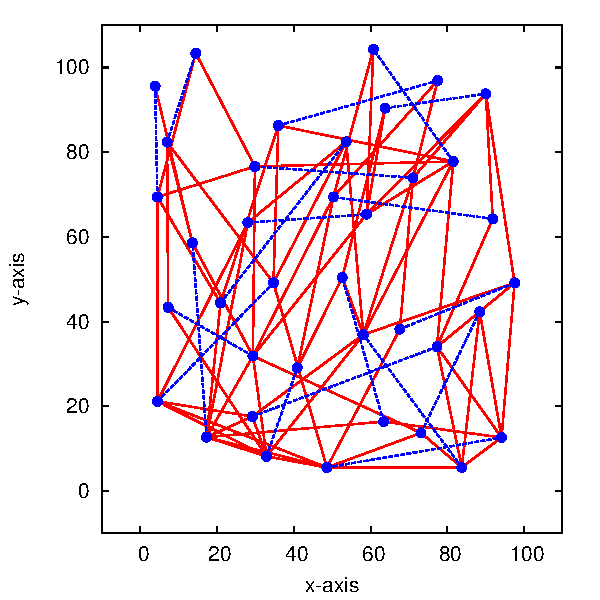
\includegraphics[scale=0.25]{figure-topo.pdf}
}
\hspace{0.05pt}
\subfigure[After]
{
	\rotatebox[origin=c]{180} { 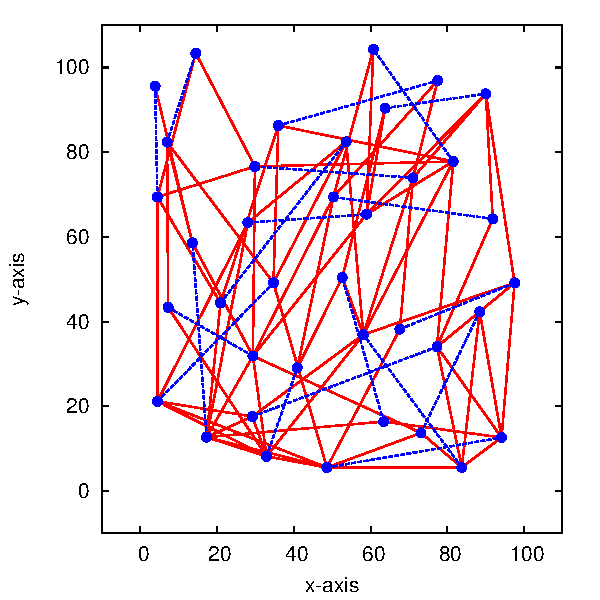
\includegraphics[scale=0.25]{figure-topo.pdf} }
}
\caption{Side by side figures with rotation}
\label{fig:rotation}
\end{figure}

\tableofcontents
\listoffigures
\listoftables

\end{document}